\documentclass[letter,10pt]{sig-alternate-10pt}

\usepackage{graphicx}
\usepackage{subfigure}

\usepackage{ifpdf}
\ifpdf
\setlength{\pdfpagewidth}{8.5in}
\setlength{\pdfpageheight}{11in}
\else
\fi

\begin{document}

\title{EMD + sensor data}

\numberofauthors{2}
\author{
% 1st. author
\alignauthor
Romain Fontugne\\
       \affaddr{The University of Tokyo / JFLI, CNRS}
% 2nd. author
\alignauthor
Jorge Ortiz\\
       \affaddr{University of California, Berkeley}
\and  % use '\and' if you need 'another row' of author names
% 3rd. author
\alignauthor
David Culler\\
       \affaddr{University of California, Berkeley}
% 4th. author
\alignauthor 
Hiroshi Esaki\\
       \affaddr{The University of Tokyo}
}

\maketitle

% % A category with the (minimum) three required fields
% \category{H.4}{Information Systems Applications}{Miscellaneous}
% %A category including the fourth, optional field follows...
% \category{D.2.8}{Software Engineering}{Metrics}[complexity measures, performance measures]
% 
% \terms{Delphi theory}
% 
% \keywords{ACM proceedings, \LaTeX, text tagging}

\begin{abstract}
here comes the abstract, blablabla...

a

b

o

u

t

1

5

0

w

o

r

d

s
\end{abstract}

\section{Introduction}
Green IT

Understand the energy consumption of a building and identify savings opportunities.

Identification of energy consuming devices that are correlated.
Uncover usage patterns of correlated device that are energy efficient.
Detect deviation from the energy efficient pattern and report to the user.

During the design of our application the first difficulty was to identify the set of devices that have related energy consumption.

This article focuses on this problem

\newpage

\section{Dataset}
The intent of the Green University of Tokyo Project (GUTP) \cite{gutp} is to reduce the university environmental impacts associated to its electric energy consumption.
The first step of this project was to deploy sensors at the Building No.2 of the Faculty of Engineering 
Electric power consumption of a 12 floors building containing researchers office and classroom.
1215 sensors monitoring different devices...

received attention in the past \cite{ogawa:lncs2011}.

Focus on a simple example: 3 weeks during the summer 2011 (from July 4th to July 24th)
includes one day holiday (July 18th)
3 different sensors:
\begin{itemize}
 \item 2 are measuring the electric power consumption of two devices from the same room. Electric Heat Pump and the room lighting system.
 \item 1 is measuring the electric power consumption of a Gas Heat Pump that is heating and cooling a different room in the same building.
\end{itemize}

\section{Problem statement}\label{problem}
Find device correlation at large spatial and time scales.

Usual measures on sensor data like correlation coefficient or granger causality \cite{kim:buildsys2010}
-- this is not working


\begin{figure}
 \subfigure[EHP]{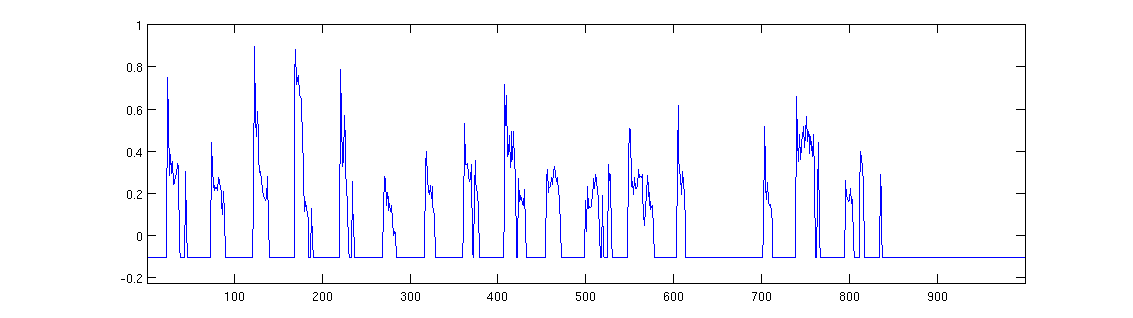
\includegraphics[width=.5\textwidth]{img/25.png}}
 \subfigure[Light]{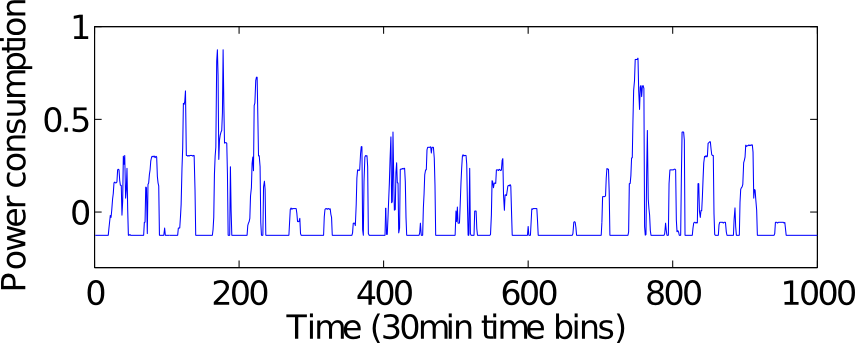
\includegraphics[width=.5\textwidth]{img/26.png}}
 \subfigure[GHP]{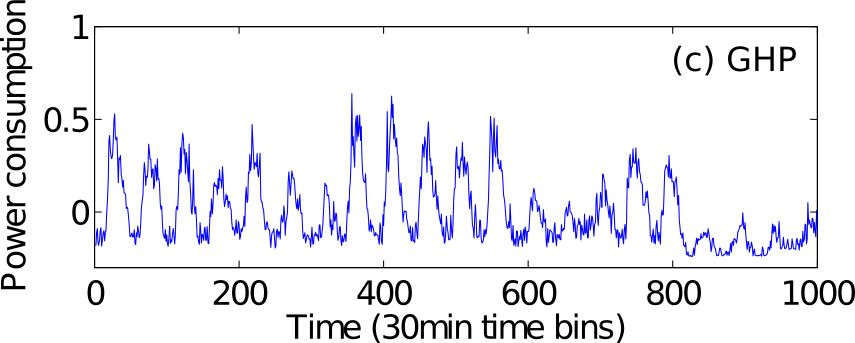
\includegraphics[width=.5\textwidth]{img/41.png}}
 \caption{Data from three different sensors captured in 2011 from July 4th to July 24th.}
 \label{fig:raw}
\end{figure}

For example correlation coefficients for the 3 signals...
correlation coefficient for the EHP and Light signals: $0.772013$
correlation coefficient for the EHP and GHP signals: $0.636967$

These scores suggest that the EHP signal is related to the two other measured signals.

These results were expected for the EHP and Light signals as the two measured devices operate for the same room and are used simultaneously.
These results, however, suggest that the EHP and GHP signals are highly correlated whereas in facts the two corresponding devices are located at two opposite sides of the building and their functioning is independent.
The small difference between the two computed correlation coefficients is misleading as one could conclude that the three signals are correlated and the corresponding devices are activated by a single action.

The high correlation coefficients obtained for these three signals result .... weekly pattern....
small difference = local fluctuation...

this high score comes from the fact that the two devices are monitoring offices that are weekly used.

Indeed the weekly pattern of the data trump the correlation coefficients....

How to inspect only the local fluctuations...?
we'd like to have an elegant solution (i.e. not specifying the interesting time scale)


\newpage

\section{Methodology}\label{method}
Remove the weekly trend of the data to analyze the detailed changes that convey the device behavior at small time scales.

\subsection{Empirical Mode Decomposition}

Empirical Mode Decomposition (EMD) \cite{huang:emd1998} is a recent techniques used for de-treding...

non-stationary non-linear signal

TODO explanation of EMD


intrinsic mode functions (IMFs)

In order to ensure that the IMFs corresponding to two distinct signals the EMD decomposition is 
We use bivariate EMD \cite{rilling:biemd2007} to decompose two signals at once and obtain their IMF at the same time scale.

\begin{figure*}
 \subfigure[EHP vs. Light]{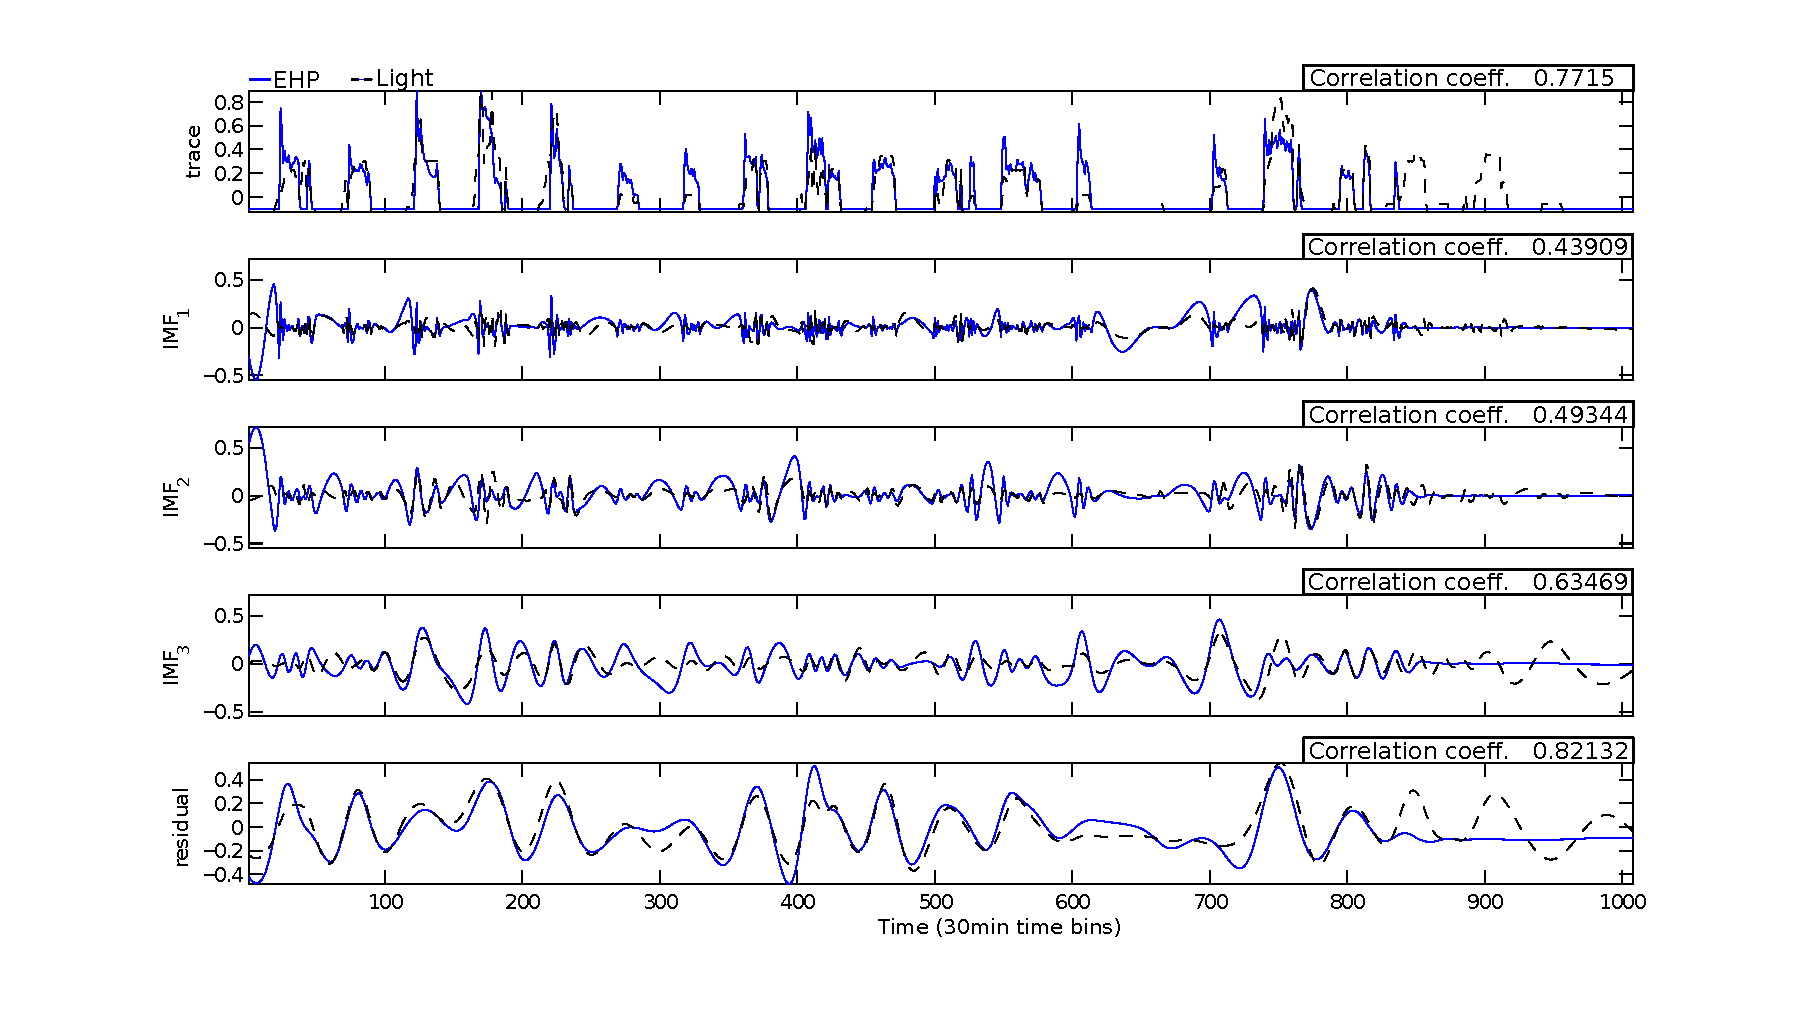
\includegraphics[width=\textwidth]{img/emd_25_26.eps}}
 \subfigure[EHP vs. GHP]{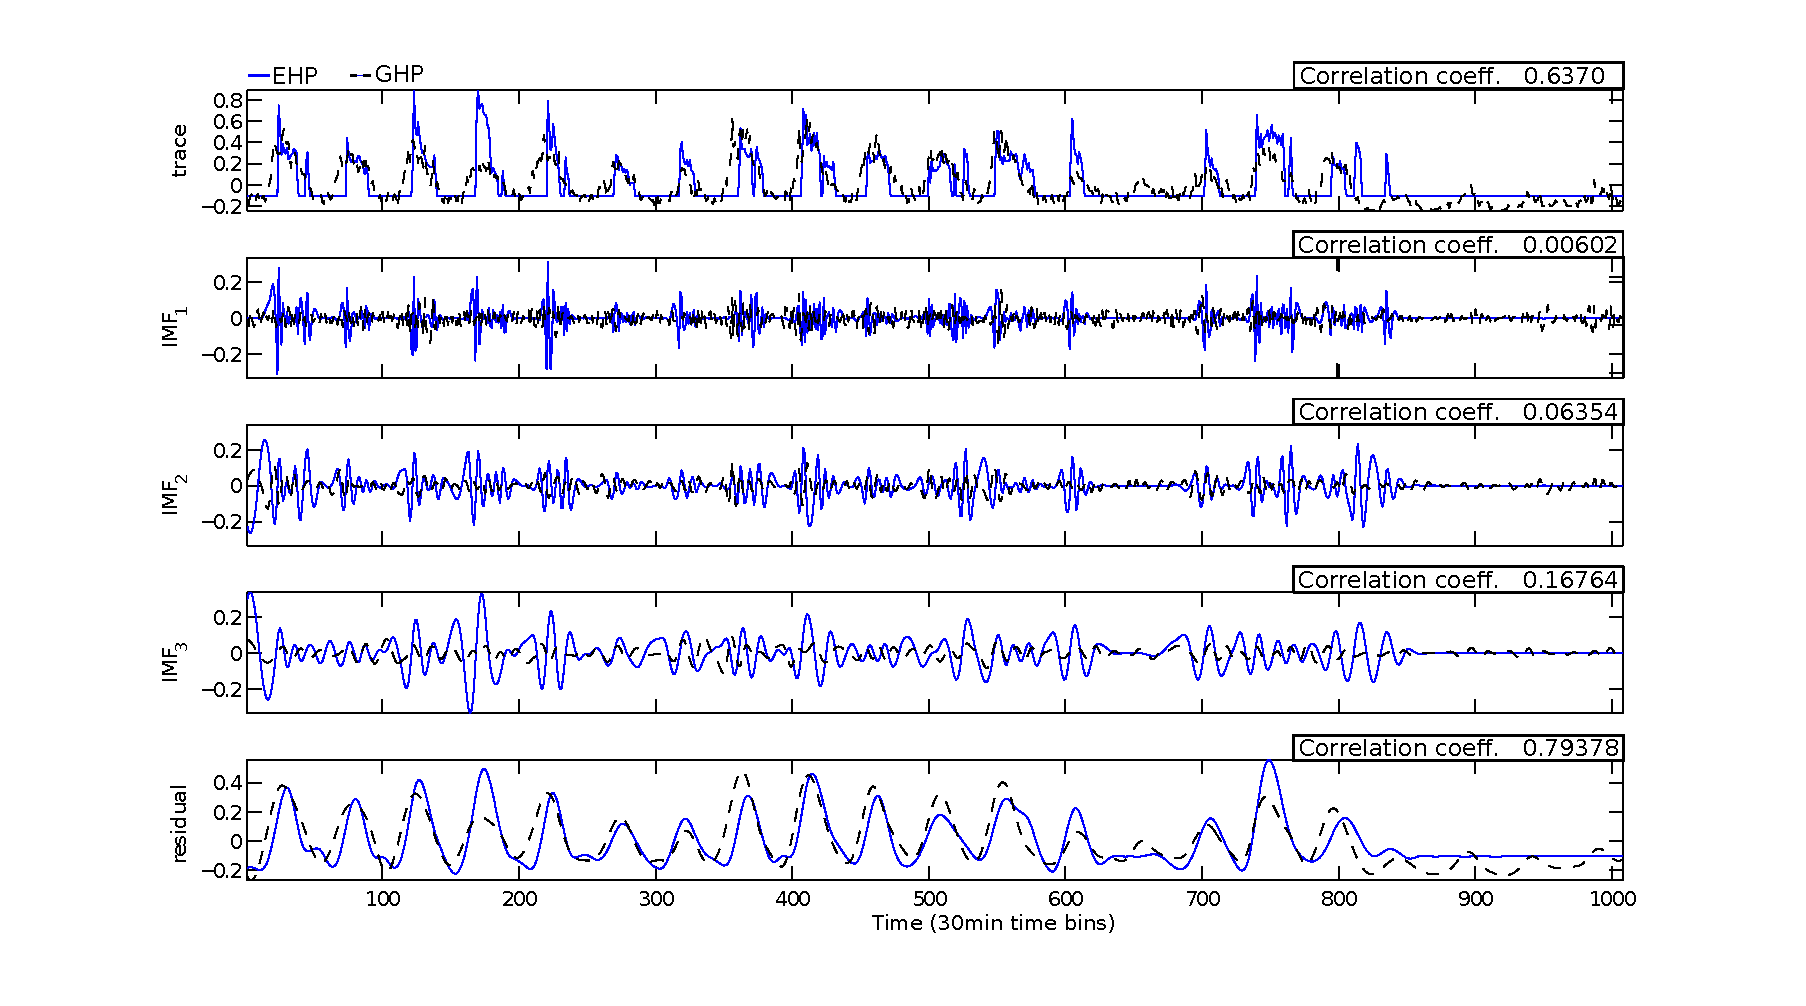
\includegraphics[width=\textwidth]{img/emd_25_41.eps}}
 \caption{Empirical Mode Decomposition}
 \label{fig:raw}
\end{figure*}

\newpage

\section{Results}
EMD on the 3 signals introduced in Section \ref{problem}
Using EMD we show that the 3 signals have a common weekly pattern, however, only two signals are correlated at smaller time scales.

\subsection{Data de-trending}
\begin{table*}
\begin{center}
\begin{tabular}{|l|l|l|l|l|l|}
\hline
× & Original data & 1st IMF & 2nd IMF & 3rd IMF & Residual\\ \hline
EHP, Light & 0.7720 & 0.4431 & 0.5104 & 0.6171 & 0.8114\\ \hline
EHP, GHP & 0.6369 & -0.0055 & 0.0883 & 0.2350 & 0.7956\\ \hline
\end{tabular}

\caption{Correlation coefficients of the analyzed signal and their IMF uncovered by EMD}

\end{center}
\end{table*}

Speak about the three IMFs and their correlation coefficients.

\subsection{Discussion}
EMD works perfectly although the weekly pattern of the data is altered the last analyzed week.

EMD inherently finds the interesting time scales.

number of zero crossing = mean frequency/time scale:
  TODO give the time scale for each IMF.


\section{Conclusion}
what is our problem

what we did

contributions and main results

future works

\section*{Acknowledgments}
The authors thanks ....(Patrick, Patrice, Pierre for EMD, Ochiai-san for the data, Kensuke, Young for discussion)
This research was partially supported by the JSPS fellowship program.

\bibliographystyle{abbrv}
\bibliography{references}

\end{document}
